\documentclass{../res/univ-projet}

%Import des packages utilisés pour le document
\usepackage[utf8x]{inputenc}
\usepackage[francais]{babel}
\usepackage[T1]{fontenc}
%\usepackage{array}
%\usepackage{hyperref}
%\usepackage{tabularx, longtable}
%\usepackage[table]{xcolor}
%\usepackage{fancyhdr}
%\usepackage{lastpage}

\definecolor{gris}{rgb}{0.95, 0.95, 0.95}

%Redéfinition des marges
%\addtolength{\hoffset}{-2cm}
%\addtolength{\textwidth}{4cm}
\addtolength{\topmargin}{-1cm}
\addtolength{\textheight}{1cm}
\addtolength{\headsep}{0.8cm} 
\addtolength{\footskip}{-0.2cm}


%Import page de garde et structures pour la gestion de projet
%\usepackage{structures}

%Variables
\logo{../res/logo_univ.png}
\title{Cahier des Recettes}
\author{Pierre \bsc{Balmelle}, Lucas \bsc{Barbay}}
\projet{Projet PGP}
\projdesc{Etude et implantation d'un outil graphique de gestion de clé PGP}
\filiere{Master 1 SSI }
\matiere{Conduite de projet}
\version{0.6}
\relecteur{Olivier \bsc{Thibault}}
\signataire{}
\date{\today}


\histentry{0.6}{07/03/2015}{Ajout des tests de non-régression.}
\histentry{0.5}{15/12/2014}{Respect de la STB v0.4 et ajout des données de test.}
\histentry{0.4}{05/12/2014}{Ajout de toutes les procédures liées aux commandes GPG.}
\histentry{0.3}{24/11/2014}{Respect de la STB v0.3.}
\histentry{0.2}{15/11/2014}{Ajout des parties Introduction, Documents applicables et de référence, Environnement de test, Responsabilités,
Stratégie de tests, Gestion des anomalies.}
\histentry{0.1}{31/10/2014}{Version initiale.}


% -- Début du document -- %
\begin{document}

%Page de garde
\maketitle
\newpage
%La table des matières
\tableofcontents
\newpage

\section{Introduction}

% Présentation succinte du sujet et hyp de travail.
Ce document est le Cahier de Recette (CDR) de la réalisation d'une interface graphique pour le logiciel GnuPG.
Cette interface permettra d'utiliser complètement l'outil OpenPGP de façon intuitive et pédagogique de façon 
à être accessible même par des personnes ayant des connaissances limitées dans le domaine de l'informatique. 

\subsection{Fonctionnalités du logiciel}
Le logiciel est une interface graphique pour le GnuPG (implémentation GNU du standart OpenPGP).
Les différents cas d'utilisations :
\begin{itemize}
 \item Exécuter une action GPG.
 \item Affichage des commandes et des erreurs.
 \item Choix du fichier de configuration.
 \item Attaque sur la seconde pré-image.
\end{itemize}

\subsection{Liste des objets à tester}
Nous avons dégagé 2 objets à tester : 
\begin{itemize}
 \item L'interface graphique des fonctions GnuPG.
 \item L'implémentation de l'attaque sur les secondes pré-images. 
\end{itemize}

L'interface graphique permettra d'utiliser chaque commande et option de GPG et ce de façon le plus intuitif possible. Nous
devrons tester le résultat des commandes ainsi que le temps d'exécution pour satisfaire le client en terme de fluidité de l'interface.

Enfin, il nous faudra tester l'implémentation de l'attaque. 


\section{Documents applicables et de référence}
% Liste des
% - Références des documents quidefinissent formellement les principes
%   directeurs et le hypothèse de travail prise en compte pour l'établissement de la spécification.
% - Références des documents cités dans la STB au titre d'explication ou de justification.
Différents documents de référence :
\begin{itemize}
\item Définitions du standard OpenPGP \href{file:../../ressources/openPGP/rfc4880-en.pdf}{RFC 4880}
  et \href{file:../../ressources/openPGP/rfc2440-fr.pdf}{RFC 2440}.
\item Le logiciel \href{https://www.gnupg.org/}{GnuPG} (GNU Privacy Guard) implantation Open Source
  de OpenPGP.
\item Editeurs graphiques existant
  (\href{http://www.gnupg.org/related_software/frontends.en.html}{KGpg, GPA, Seahorse}).
\end{itemize}

\section{Terminologie et sigles utilisés}
\textcolor{blue}{
  Le glossaire est dans un fichier à part, il est commun aux autres documents de gestion de projet.
}

\section{Environnement de test}
\subsection{Sites de réalisation des tests}
Les test seront réalisés soit sur le site de l'université soit au domicile des deux testeurs sur leur machine personnelle.



\subsection{Configurations matérielles utilisées}
Voici la configuration des machines personnelles des deux testeurs :
\begin{itemize}
 \item PC n°1 : Un ordinateur portable équipé de Xubuntu 64 bits avec un processeur Intel i5-3210M @ 2.50GHz et 6Go de RAM.
 \item PC n°2 : Un ordinateur portable équipé de Xubuntu 64 bits avec un processeur Intel i7-2630QM @ 2.00 GHz et 6Go de RAM.
\end{itemize}
Seront également utilisées des machines virtuelles pour répondre aux besoins du client sur la compatibilité de l'interface (KDE et GNOME).

\subsection{Outils de tests mis en oeuvre}
Nous avons décidé d'utiliser le framework Qt pour réaliser ce projet. C'est donc le module Qttest de Qt que l'on a choisi car il permet de réaliser simplement les tests unitaires et benchmark.

\subsection{Jeux de données/Bases de données}
Nous aurons comme jeu de données les différentes clés contenues dans le trousseau de test.


\subsection{Contraintes à prendre en compte}
Chaque procédure de test devra être réalisée sous KDE et sous GNOME.
Les tests unitaires et de non-régression seront réalisés à l'aide de l'api Qt (automatiquement), et les tests d'intégration à l'aide de l'interface (manuellement).



\section{Responsabilités}

  La création et la gestion des procédures de test sera effectuée par les responsables qualité de l'équipe. Chaque équipe travaillant au développement d'un composant est chargée de tester celui-ci continuellement et de publier les résultats des tests.
  
  Afin d'assurer la compréhension générale du code source, toute l'équipe peut et est encouragée à signaler une anomalie détectée au cours du développement : soit elle est résolue par la même personne/groupe, soit cette personne/ce groupe transmet les résultats 
  des tests à une autre personne/groupe afin que celle-ci travaille à la réparation de l'anomalie.
  
  À tout moment une équipe peut reporter des anomalies dans une procédure de test. Dans ce cas, les responsables techniques concernés travailleront à améliorer la procédure incriminée et diffuseront les mises à jour à l'ensemble de l'équipe.

  Dans tous les cas, les instructions incluses dans la partie \emph{Gestion des anomalies} sont à respecter.


\section{Stratégies de tests}

\subsection{Description de l'approche et des phases de test}
Dès qu'un test pour un composant sera réalisable, il sera fait. Ces tests devront être appliqués à chaque nouvelle version du composant.


\subsection{Campagne de test}

Les différentes campagnes de tests correspondront aux livrables envoyés au client.

\subsection{Ordre d'exécution des tests}

L'ordre d'exécution des tests suivra l'ordre du plan de développement.

\subsection{Critères d'arrêt des tests}

Un test est considéré comme échoué dès qu'une de ses étapes échoue, produit un résultat non attendu ou est impossible à mener à bout.


\section{Gestion des anomalies}

Quand des anomalies seront détectées, la procédure suivante devra être respectée:
  \begin{itemize}
   \item Création d'un mémo précisant l'anomalie rencontrée ainsi que les conditions de reproduction de l'anomalie si disponibles et l'état du système lors de l'apparition de l'anomalie.  
   Un identifiant unique lui sera attribué.
   \item Ajout d'une entrée au journal de test précisant la date du test, la référence du mémo, le nom ainsi que la référence de l'exigence de 
   qualité non respectée.
   \item Diffusion de la note à l'équipe de développement.
   \item Une personne est désignée pour corriger l'anomalie.
   \item Cette personne vérifie la gravité de l'anomalie, puis la corrige.
   \item Une deuxième personne s'assure que l'anomalie est bien corrigée.
   \item Une fois la vérification effectuée, la personne ayant corrigé l'anomalie établit un contre-mémo portant le même identifiant et précisant les raisons supposées 
   de l'anomalie ainsi que les corrections mises en place.
  \end{itemize}
  

  Dans la pratique, la gestions des anomalies sera faite à l'aide de l'outil \emph{issue tracker} de
  la plate-forme d'hébergement Gitlab. Cet outil permet la création de files de discussion associées à un bug
  de l'application. Il laisse aussi la possibilité aux collaborateurs du projet de prendre en charge 
  une \emph{issue} particulière. L'ensemble des \emph{issues} ouvertes est conservé par Gitlab ainsi
  que les files de discussion associés permettant de parcourir l'historique des bugs du projet.


\section{Procédures de test}

\subsection{Types de tests}

  Les différents types de tests utilisés sont :
  \begin{itemize}
   \item Les tests unitaires, préfixés par u,
   \item Les tests de non-régression, préfixés par nr,
   \item Les tests d'intégration, préfixés par i.
  \end{itemize}
  

\subsection{Tests unitaires}

\begin{center}
    %---------------------------------------Test N° U1------------------------------------------------------------------------------
    \begin{tabular}{|c|p{5cm}|p{5cm}|p{1.5cm}|p{1.5cm}|}
      \hline
      \multicolumn{3}{|l|}{Objet testé : Interface Graphique} & \multicolumn{2}{c|}{Version : 0.1}\\ \hline
      \multicolumn{5}{|l|}{Objectif de test : Création de clé}\\ \hline
      \multicolumn{3}{|l|}{Procédure n° U1} & \multicolumn{2}{p{3cm}|}{Pré-requis : }\\ \hline
      \multicolumn{1}{|c|}{N°} & \multicolumn{1}{c|}{Actions} & \multicolumn{1}{c|}{Résultats attendus} & 
      \multicolumn{1}{c|}{Exigence} & \multicolumn{1}{c|}{OK/KO}\\ \hline
      1 & Créer une clé a & La clé a été créée &  & NOK \\
      2 &  &  &  & \\
      3 &  &  &  & \\ 
      4 &  &  &  & \\
      5 &  &  &  & \\
      6 &  &  &  & \\
      7 &  &  &  & \\
      8 &  &  &  & \\
      9 &  &  &  & \\
      10 &  &  &  &\\ 
	\hline
    \end{tabular}
    \vskip 2.2cm


 %---------------------------------------Test N° U2------------------------------------------------------------------------------
    \begin{tabular}{|c|p{5cm}|p{5cm}|p{1.5cm}|p{1.5cm}|}
      \hline
      \multicolumn{3}{|l|}{Objet testé : Attaque seconde pré-image} & \multicolumn{2}{c|}{Version : 0.1}\\ \hline
      \multicolumn{5}{|l|}{Objectif de test : La clé produite a la même seconde pré-image que celle donnée.}\\ \hline
      \multicolumn{3}{|l|}{Procédure n° U2} & \multicolumn{2}{p{3cm}|}{Pré-requis : }\\ \hline
      \multicolumn{1}{|c|}{N°} & \multicolumn{1}{c|}{Actions} & \multicolumn{1}{c|}{Résultats attendus} & 
      \multicolumn{1}{c|}{Exigence} & \multicolumn{1}{c|}{OK/KO}\\ \hline
      1 & Donner une clé publique au programme d'attaque & Le programme renvoie une clé différente avec la même pré-image &  & NOK \\
      2 & Comparer la clé produite avec la clé initiale & Les deux clés ont la même seconde pré-image &  & NOK \\
      3 &  &  &  & \\ 
	  4 &  &  &  & \\
      5 &  &  &  & \\
	  6 &  &  &  & \\
      7 &  &  &  & \\
      8 &  &  &  & \\
      9 &  &  &  & \\
      10 &  &  &  &\\ 
	\hline
    \end{tabular}
    \vskip 2.2cm





 %---------------------------------------Test N° U3------------------------------------------------------------------------------
    \begin{tabular}{|c|p{5cm}|p{5cm}|p{1.5cm}|p{1.5cm}|}
      \hline
      \multicolumn{3}{|l|}{Objet testé : GuiPG} & \multicolumn{2}{c|}{Version : 0.3}\\ \hline
      \multicolumn{5}{|l|}{Objectif de test : Tester les classes liées à la gestion de profil}\\ \hline
      \multicolumn{3}{|l|}{Procédure n° U3} & \multicolumn{2}{p{3cm}|}{Pré-requis : }\\ \hline
      \multicolumn{1}{|c|}{N°} & \multicolumn{1}{c|}{Actions} & \multicolumn{1}{c|}{Résultats attendus} & 
      \multicolumn{1}{c|}{Exigence} & \multicolumn{1}{c|}{OK/KO}\\ \hline
      1 & Demander la liste des profils & On récupère une liste de profils &  & OK \\
      2 & Créer un profil & Le profil est créé &  & OK \\
      3 & Supprimer ce profil & Le profil est supprimé &  & OK \\ 
      4 & Demander la liste des profils & La même liste est renvoyée qu'au début &  & OK \\
      5 &  &  &  & \\
      6 &  &  &  & \\
      7 &  &  &  & \\
      8 &  &  &  & \\
      9 &  &  &  & \\
      10 &  &  &  &\\ 
  \hline
    \end{tabular}
    \vskip 2.2cm


 %---------------------------------------Test N° U4------------------------------------------------------------------------------
    \begin{tabular}{|c|p{5cm}|p{5cm}|p{1.5cm}|p{1.5cm}|}
      \hline
      \multicolumn{3}{|l|}{Objet testé : Classe KeyImport} & \multicolumn{2}{c|}{Version : 0.5}\\ \hline
      \multicolumn{5}{|l|}{Objectif de test : Test de la classe}\\ \hline
      \multicolumn{3}{|l|}{Procédure n° U4} & \multicolumn{2}{p{3cm}|}{Pré-requis : }\\ \hline
      \multicolumn{1}{|c|}{N°} & \multicolumn{1}{c|}{Actions} & \multicolumn{1}{c|}{Résultats attendus} & 
      \multicolumn{1}{c|}{Exigence} & \multicolumn{1}{c|}{OK/KO}\\ \hline
      1 & Créer une instance de la classe &  &  & NOK \\
      2 & Utiliser la fonction importFunction & L'affichage des clés est modifié et affiche les nouvelles clés si il y en a &  & NOK \\
      3 &  &  &  & \\
      4 &  &  &  & \\
      5 &  &  &  & \\
	    6 &  &  &  & \\
      7 &  &  &  & \\
      8 &  &  &  & \\
      9 &  &  &  & \\
      10 &  &  &  &\\ 
	\hline
    \end{tabular}
    \vskip 2.2cm
    
        %---------------------------------------Test N° U5------------------------------------------------------------------------------
    \begin{tabular}{|c|p{5cm}|p{5cm}|p{1.5cm}|p{1.5cm}|}
      \hline
      \multicolumn{3}{|l|}{Objet testé : Classe Profile} & \multicolumn{2}{c|}{Version : 0.5}\\ \hline
      \multicolumn{5}{|l|}{Objectif de test : Test de la classe}\\ \hline
      \multicolumn{3}{|l|}{Procédure n° U5} & \multicolumn{2}{p{3cm}|}{Pré-requis : }\\ \hline
      \multicolumn{1}{|c|}{N°} & \multicolumn{1}{c|}{Actions} & \multicolumn{1}{c|}{Résultats attendus} & 
      \multicolumn{1}{c|}{Exigence} & \multicolumn{1}{c|}{OK/KO}\\ \hline
      1 & Créer une instance de la classe &  &  & OK \\
      2 & Utiliser la fonction getId & La fonction renvoie l'id donnée au constructeur &  & OK \\
      3 & Utiliser la fonction setConfigurationPath &  &  & OK \\
      4 & Utiliser la fonction getConfigurationPath & La fonction renvoie le path donné à l'étape précédente &  & OK \\
      5 & Utiliser la fonction setGPGExecutable &  &  & OK \\
      6 & Utiliser la fonction getGPGExecutable & La fonction renvoie le path donné à l'étape précédente &  & OK \\
      7 & Utiliser la fonction getName & La fonction renvoie le nom donné au constructeur &  & OK \\
      8 &  &  &  &  \\
      9 &  &  &  & \\
      10 &  &  &  &\\ 
  \hline
    \end{tabular}
    \vskip 2.2cm
    
	
%---------------------------------------Test N° U6------------------------------------------------------------------------------
    \begin{tabular}{|c|p{5cm}|p{5cm}|p{1.5cm}|p{1.5cm}|}
      \hline
      \multicolumn{3}{|l|}{Objet testé : Classe Launcher} & \multicolumn{2}{c|}{Version : 0.5}\\ \hline
      \multicolumn{5}{|l|}{Objectif de test : Test de la classe}\\ \hline
      \multicolumn{3}{|l|}{Procédure n° U6} & \multicolumn{2}{p{3cm}|}{Pré-requis : }\\ \hline
      \multicolumn{1}{|c|}{N°} & \multicolumn{1}{c|}{Actions} & \multicolumn{1}{c|}{Résultats attendus} & 
      \multicolumn{1}{c|}{Exigence} & \multicolumn{1}{c|}{OK/KO}\\ \hline
      1 & Créer une instance de la classe &  &  & OK \\
      2 & Utiliser la fonction alreadyRun & La fonction renvoie false &  & OK \\
      3 & Utiliser la fonction run & Une exception IllegalArgumentException est levée &  & OK \\
      4 & Utiliser la fonction addMainWindow avec un argument à NULL & Une exception IllegalArgumentException est levée &  & OK \\
      5 & Utiliser la fonction addMainWindow & &  & OK \\
	    6 & Utiliser la fonction run &  &  & OK \\
      7 & Utiliser la fonction alreadyRun & La fonction renvoie true &  & OK \\
      8 & Utiliser la fonction profileIsLoad avec le même Profile que pour addMainWindow & La fonction ne renvoie pas NULL &  & OK \\
      9 & Utiliser la fonction unloadProfileWithWindow avec le même Profile que pour addMainWindow &  &  & OK \\
      10 & Utiliser la fonction stop &  &  & OK \\
      11 & Utiliser la fonction alreadyRun & La fonction renvoie false &  & OK \\ 
	\hline
    \end{tabular}
    \vskip 2.2cm
	
	
%---------------------------------------Test N° U7------------------------------------------------------------------------------
    \begin{tabular}{|c|p{5cm}|p{5cm}|p{1.5cm}|p{1.5cm}|}
      \hline
      \multicolumn{3}{|l|}{Objet testé : Classe Action} & \multicolumn{2}{c|}{Version : 0.5}\\ \hline
      \multicolumn{5}{|l|}{Objectif de test : Test de la classe}\\ \hline
      \multicolumn{3}{|l|}{Procédure n° U7} & \multicolumn{2}{p{3cm}|}{Pré-requis : }\\ \hline
      \multicolumn{1}{|c|}{N°} & \multicolumn{1}{c|}{Actions} & \multicolumn{1}{c|}{Résultats attendus} & 
      \multicolumn{1}{c|}{Exigence} & \multicolumn{1}{c|}{OK/KO}\\ \hline
      1 & Créer une instance de la classe &  &  & OK \\
      2 & Utiliser la fonction getCmd & La fonction renvoie la commande donnée au constructeur &  & OK \\
      3 & Utiliser la fonction getOptions & La fonction renvoie les options données au constructeur &  & OK \\
      4 & Utiliser la fonction getInteractions & La fonction renvoie les interactions donnés au constructeur &  & OK \\
      5 & Utiliser la fonction getArgs & La fonction renvoie les arguments donnés au constructeur &  & OK \\
	    6 & Utiliser la fonction hasInteractions & La fonction renvoie true si des interactions ont été données au constructeur, false sinon &  & OK \\
      7 & Utiliser la fonction nextInteraction autant de fois que le nombre d'interactions données au constructeur plus une & La fonction renvoie un QString contenant une interaction à chaque appel à la fonction, et NULL au dernier &  & OK \\
      8 &  &  &  & \\
      9 &  &  &  & \\
      10 &  &  &  &\\ 
	\hline
    \end{tabular}
    \vskip 2.2cm
	
%---------------------------------------Test N° U8------------------------------------------------------------------------------
    \begin{tabular}{|c|p{5cm}|p{5cm}|p{1.5cm}|p{1.5cm}|}
      \hline
      \multicolumn{3}{|l|}{Objet testé : Classe GPGManager} & \multicolumn{2}{c|}{Version : 0.5}\\ \hline
      \multicolumn{5}{|l|}{Objectif de test : Test de la classe}\\ \hline
      \multicolumn{3}{|l|}{Procédure n° U8} & \multicolumn{2}{p{3cm}|}{Pré-requis : }\\ \hline
      \multicolumn{1}{|c|}{N°} & \multicolumn{1}{c|}{Actions} & \multicolumn{1}{c|}{Résultats attendus} & 
      \multicolumn{1}{c|}{Exigence} & \multicolumn{1}{c|}{OK/KO}\\ \hline
      1 & Créer une instance de la classe &  &  & OK \\
      2 & Utiliser la fonction setAction &  &  & OK \\
      3 & Utiliser la fonction execute &  &  & OK \\
      4 & Attendre le signal finished & Le signal finished est reçu &  & OK \\
      5 & Utiliser la fonction getOutput & La fonction renvoie le texte renvoyé par gpg quand gpg exécute l'action donnée en argument à setAction &  & OK \\
	    6 & &  &  &  \\
      7 &  &  &  &  \\
      8 &  &  &  &  \\
      9 &  &  &  & \\
      10 &  &  &  & \\ 
	\hline
    \end{tabular}
    \vskip 2.2cm
	

%---------------------------------------Test N° U9------------------------------------------------------------------------------
    \begin{tabular}{|c|p{5cm}|p{5cm}|p{1.5cm}|p{1.5cm}|}
      \hline
      \multicolumn{3}{|l|}{Objet testé : Classe GPGKey} & \multicolumn{2}{c|}{Version : 0.5}\\ \hline
      \multicolumn{5}{|l|}{Objectif de test : Test de la classe}\\ \hline
      \multicolumn{3}{|l|}{Procédure n° U9} & \multicolumn{2}{p{3cm}|}{Pré-requis : }\\ \hline
      \multicolumn{1}{|c|}{N°} & \multicolumn{1}{c|}{Actions} & \multicolumn{1}{c|}{Résultats attendus} & 
      \multicolumn{1}{c|}{Exigence} & \multicolumn{1}{c|}{OK/KO}\\ \hline
      1 & Créer une instance de la classe &  &  & NOK \\
      2 & Utiliser la fonction getSubKeys & La fonction renvoie une QList<GPGKey> correspondant aux sous-clés de la clé donnée au constructeur &  & NOK \\
      3 & Utiliser la fonction getEmail & La fonction renvoie un QString correspondant à l'email associé à la clé donnée au constructeur &  & NOK \\
      4 & Utiliser la fonction getName & La fonction renvoie un QString correspondant au nom associé à la clé donnée au constructeur &  & NOK \\
      5 & Utiliser la fonction getDate & La fonction renvoie une QDate correspondant à la date de création de la clé donnée au constructeur &  & NOK \\
      6 & Utiliser la fonction getId & La fonction renvoie un QString correspondant au keyID de la clé donnée au constructeur &  & NOK \\
      7 & Utiliser la fonction getComments & La fonction renvoie un QString correspondant au commentaire associé à la clé donnée au constructeur &  & NOK \\
      8 & Utiliser la fonction getTrust & La fonction renvoie un GPGKeyLevel correspondant au niveau de confiance de la clé donnée au constructeur &  & NOK \\
      9 & Utiliser la fonction addSubKey, puis la fonction getSubKeys & La fonction getSubKeys renvoie une QList<GPGKey> contenant la clé donnée à addSubKey &  & NOK \\
      10 & Utiliser la fonction removeSubKey, puis la fonction getSubKeys & La fonction getSubKeys renvoie une QList<GPGKey> ne contenant pas la clé donnée à addSubKey &  & NOK \\ 
      11 & Utiliser la fonction setTrust, puis la fonction getTrust & La fonction getTrust renvoie un GPGKeyLevel contenant au niveau donné à setTrust &  & NOK \\ 
  \hline
    \end{tabular}
    \vskip 2.2cm

%---------------------------------------Test N° U10------------------------------------------------------------------------------
    \begin{tabular}{|c|p{5cm}|p{5cm}|p{1.5cm}|p{1.5cm}|}
      \hline
      \multicolumn{3}{|l|}{Objet testé : Classe MainWindowModel} & \multicolumn{2}{c|}{Version : 0.5}\\ \hline
      \multicolumn{5}{|l|}{Objectif de test : Test de la classe}\\ \hline
      \multicolumn{3}{|l|}{Procédure n° U10} & \multicolumn{2}{p{3cm}|}{Pré-requis : }\\ \hline
      \multicolumn{1}{|c|}{N°} & \multicolumn{1}{c|}{Actions} & \multicolumn{1}{c|}{Résultats attendus} & 
      \multicolumn{1}{c|}{Exigence} & \multicolumn{1}{c|}{OK/KO}\\ \hline
      1 & Créer une instance de la classe &  &  & OK \\
      2 & Utiliser la fonction getLauncher & La fonction renvoie le Launcher donné au constructeur &  & OK \\
      3 & Utiliser la fonction getGuiPGApp & La fonction renvoie le GuiPGApp donné au constructeur &  & OK \\
      4 & Utiliser la fonction getConf & La fonction renvoie la Configuration donnée au constructeur &  & OK \\
      5 & Utiliser la fonction getProfile & La fonction renvoie le Profile donné au constructeur &  & OK \\
      6 & Utiliser la fonction loadProfile &  &  & OK \\
      7 & Utiliser la fonction initKeyManager &  &  & OK \\
      8 & Utiliser la fonction getKeyManager & La fonction renvoie un KeyManager &  & OK \\
      9 &  &  &  &  \\
      10 &  &  &  &  \\ 
  \hline
    \end{tabular}
    \vskip 2.2cm


    %---------------------------------------Test N° U11------------------------------------------------------------------------------
    \begin{tabular}{|c|p{5cm}|p{5cm}|p{1.5cm}|p{1.5cm}|}
      \hline
      \multicolumn{3}{|l|}{Objet testé : Classe KeyExport} & \multicolumn{2}{c|}{Version : 0.5}\\ \hline
      \multicolumn{5}{|l|}{Objectif de test : Test de la classe}\\ \hline
      \multicolumn{3}{|l|}{Procédure n° U11} & \multicolumn{2}{p{3cm}|}{Pré-requis : }\\ \hline
      \multicolumn{1}{|c|}{N°} & \multicolumn{1}{c|}{Actions} & \multicolumn{1}{c|}{Résultats attendus} & 
      \multicolumn{1}{c|}{Exigence} & \multicolumn{1}{c|}{OK/KO}\\ \hline
      1 & Avoir un trousseau de clés non vide &  &  & NOK \\
      2 & Créer une instance de la classe &  &  & NOK \\
      3 & Utiliser la fonction exportKey sur /tmp & Le fichier correspondant au path a été créé. &  & NOK \\
      4 & Utiliser la fonction exportKey sur un fichier non accessible en écriture & La fonction renvoie -1 &  & NOK \\
      5 & Utiliser la fonction exportKey sur un chemin inexistant & la fonction renvoie -1 &  & NOK \\
      6 & Utiliser la fonction exportKey sur un fichier déjà existant & Le fichier a été remplacé &  & NOK \\
      7 &  &  &  & \\
      8 &  &  &  & \\
      9 &  &  &  & \\
      10 &  &  &  & \\ 
  \hline
    \end{tabular}
    \vskip 2.2cm

    %---------------------------------------Test N° U12------------------------------------------------------------------------------
    \begin{tabular}{|c|p{5cm}|p{5cm}|p{1.5cm}|p{1.5cm}|}
      \hline
      \multicolumn{3}{|l|}{Objet testé : Classe KeyImport} & \multicolumn{2}{c|}{Version : 0.5}\\ \hline
      \multicolumn{5}{|l|}{Objectif de test : Test de la classe}\\ \hline
      \multicolumn{3}{|l|}{Procédure n° U12} & \multicolumn{2}{p{3cm}|}{Pré-requis : }\\ \hline
      \multicolumn{1}{|c|}{N°} & \multicolumn{1}{c|}{Actions} & \multicolumn{1}{c|}{Résultats attendus} & 
      \multicolumn{1}{c|}{Exigence} & \multicolumn{1}{c|}{OK/KO}\\ \hline
      1 & Créer une instance de la classe &  &  & NOK \\
      2 & Utiliser la fonction import sur un fichier valide & Les clés contenues dans le fichier ont été importées &  & NOK \\
      3 &  &  &  &  \\
      4 &  &  &  &  \\
      5 &  &  &  &  \\
      6 &  &  &  &  \\
      7 &  &  &  &  \\
      8 &  &  &  &  \\
      9 &  &  &  & \\
      10 &  &  &  & \\ 
  \hline
    \end{tabular}
    \vskip 2.2cm    


%TESTS D'INTEGRATION%
\subsection{Tests d'intégration}


 %---------------------------------------Test N° I1------------------------------------------------------------------------------
    \begin{tabular}{|c|p{5cm}|p{5cm}|p{1.5cm}|p{1.5cm}|}
      \hline
      \multicolumn{3}{|l|}{Objet testé : Interface graphique} & \multicolumn{2}{c|}{Version : 0.3}\\ \hline
      \multicolumn{5}{|l|}{Objectif de test : Tester la sélection du profil}\\ \hline
      \multicolumn{3}{|l|}{Procédure n° I1} & \multicolumn{2}{p{3cm}|}{Pré-requis : }\\ \hline
      \multicolumn{1}{|c|}{N°} & \multicolumn{1}{c|}{Actions} & \multicolumn{1}{c|}{Résultats attendus} & 
      \multicolumn{1}{c|}{Exigence} & \multicolumn{1}{c|}{OK/KO}\\ \hline
      1 & Lancer l'interface graphique en ligne de commande avec l'option -P & On peut choisir son profil, et en créer un si besoin &  & NOK \\
      2 & Choisir un profil & L'interface graphique s'affiche &  & NOK \\
      3 & Cliquer sur le bouton "Changer de profil" & On peut changer, créer, modifier ou supprimer un profil &  & NOK \\ 
    4 &  &  &  & \\
      5 &  &  &  & \\
    6 &  &  &  & \\
      7 &  &  &  & \\
      8 &  &  &  & \\
      9 &  &  &  & \\
      10 &  &  &  &\\ 
  \hline
    \end{tabular}
    \vskip 2.2cm

 %---------------------------------------Test N° I2------------------------------------------------------------------------------
    \begin{tabular}{|c|p{5cm}|p{5cm}|p{1.5cm}|p{1.5cm}|}
      \hline
      \multicolumn{3}{|l|}{Objet testé : Interface graphique} & \multicolumn{2}{c|}{Version : 0.3}\\ \hline
      \multicolumn{5}{|l|}{Objectif de test : Tester le mécanisme multi-instance}\\ \hline
      \multicolumn{3}{|l|}{Procédure n° I2} & \multicolumn{2}{p{3cm}|}{Pré-requis : }\\ \hline
      \multicolumn{1}{|c|}{N°} & \multicolumn{1}{c|}{Actions} & \multicolumn{1}{c|}{Résultats attendus} & 
      \multicolumn{1}{c|}{Exigence} & \multicolumn{1}{c|}{OK/KO}\\ \hline
      1 & Lancer GuiPG & GuiPG se lance &  & NOK \\
      2 & Lancer un autre GuiPG & La fenêtre de sélection de profil apparait &  & NOK \\
      3 & Sélectionner un profil non utilisé & Il y a deux fenêtres GuiPG ouvertes, chacune avec un profil différent &  & NOK \\ 
      4 & Lancer un autre GuiPG & La fenêtre de sélection de profil apparait &  & \\
      5 & Sélectionner un profil utilisé & La fenêtre GuiPG utilisant ce profil apparaît en premier plan &  & \\
      6 &  &  &  & \\
      7 &  &  &  & \\
      8 &  &  &  & \\
      9 &  &  &  & \\
      10 &  &  &  &\\ 
  \hline
    \end{tabular}
    \vskip 2.2cm


 %---------------------------------------Test N° I3------------------------------------------------------------------------------
    \begin{tabular}{|c|p{5cm}|p{5cm}|p{1.5cm}|p{1.5cm}|}
      \hline
      \multicolumn{3}{|l|}{Objet testé : Interface graphique} & \multicolumn{2}{c|}{Version : 0.3}\\ \hline
      \multicolumn{5}{|l|}{Objectif de test : Affichage des commandes et retours gpg}\\ \hline
      \multicolumn{3}{|l|}{Procédure n° I3} & \multicolumn{2}{p{3cm}|}{Pré-requis : }\\ \hline
      \multicolumn{1}{|c|}{N°} & \multicolumn{1}{c|}{Actions} & \multicolumn{1}{c|}{Résultats attendus} & 
      \multicolumn{1}{c|}{Exigence} & \multicolumn{1}{c|}{OK/KO}\\ \hline
      1 & Activer l'affichage des commandes gpg dans l'interface graphique &  &  & NOK \\
      2 & Lancer une commande gpg via l'interface graphique & La commande et les retours sont affichés &  & NOK \\
      3 &  &  &  & \\ 
      4 &  &  &  & \\
      5 &  &  &  & \\
      6 &  &  &  & \\
      7 &  &  &  & \\
      8 &  &  &  & \\
      9 &  &  &  & \\
      10 &  &  &  &\\ 
  \hline
    \end{tabular}
    \vskip 2.2cm

%TESTS DE NON REGRESSION%
\subsection{Tests de non-régression}

    %---------------------------------------Test N° NR1------------------------------------------------------------------------------
    \begin{tabular}{|c|p{5cm}|p{5cm}|p{1.5cm}|p{1.5cm}|}
      \hline
      \multicolumn{3}{|l|}{Objet testé : Classe KeyExport} & \multicolumn{2}{c|}{Version : 0.5}\\ \hline
      \multicolumn{5}{|l|}{Objectif de test : Test d'un bug rencontré}\\ \hline
      \multicolumn{3}{|l|}{Procédure n° NR1} & \multicolumn{2}{p{3cm}|}{Pré-requis : }\\ \hline
      \multicolumn{1}{|c|}{N°} & \multicolumn{1}{c|}{Actions} & \multicolumn{1}{c|}{Résultats attendus} & 
      \multicolumn{1}{c|}{Exigence} & \multicolumn{1}{c|}{OK/KO}\\ \hline
      1 & Créer une instance de la classe &  &  & NOK \\
      2 & Utiliser la fonction exportKey avec un path donné & Le fichier correspondant au path a été créé. &  & NOK \\
      3 &  &  &  & \\
      4 &  &  &  & \\
      5 &  &  &  & \\
	    6 &  &  &  & \\
      7 &  &  &  & \\
      8 &  &  &  & \\
      9 &  &  &  & \\
      10 &  &  &  &\\ 
	\hline
    \end{tabular}
    \vskip 2.2cm

%---------------------------------------Test N° NR2------------------------------------------------------------------------------
    \begin{tabular}{|c|p{5cm}|p{5cm}|p{1.5cm}|p{1.5cm}|}
      \hline
      \multicolumn{3}{|l|}{Objet testé : Classe KeyManager} & \multicolumn{2}{c|}{Version : 0.5}\\ \hline
      \multicolumn{5}{|l|}{Objectif de test : Test d'un bug rencontré lors du changement rapide de profils}\\ \hline
      \multicolumn{3}{|l|}{Procédure n° NR2} & \multicolumn{2}{p{3cm}|}{Pré-requis : }\\ \hline
      \multicolumn{1}{|c|}{N°} & \multicolumn{1}{c|}{Actions} & \multicolumn{1}{c|}{Résultats attendus} & 
      \multicolumn{1}{c|}{Exigence} & \multicolumn{1}{c|}{OK/KO}\\ \hline
      1 & Lancer GuiPG avec un profil & GuiPG se lance &  & OK \\
      2 & Créer un nouveau profil & Le nouveau profil a été créé. &  & OK \\
      3 & Changer 20 fois entre le nouveau profil et l'ancien & GuiPG ne crashe pas &  & OK \\
      4 &  &  &  & \\
      5 &  &  &  & \\
      6 &  &  &  & \\
      7 &  &  &  & \\
      8 &  &  &  & \\
      9 &  &  &  & \\
      10 &  &  &  &\\ 
  \hline
    \end{tabular}
    \vskip 2.2cm
    
\end{center}

\section{Jeux de données de test}

Les clés qui seront utilisées pour les tests se trouvent dans PrivateKeys.gpg et PublicKeys.gpg, joints dans le même dossier que ce fichier.
Elles suivent le schéma de signature décrit ci-dessous :

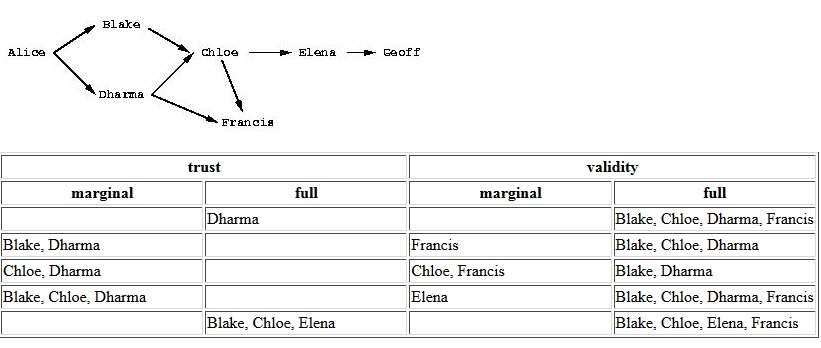
\includegraphics[scale=0.80]{graphics/trust_example.png}



\section{Couverture de test}

\begin{center}
    \begin{tabular}{|p{2.8cm}|p{4.2cm}|p{3cm}|p{5cm}|}
      \hline
      Id Exigence STB & Méthode de vérification & Procédure(s) utilisée(s) & Commentaire\\ \hline
      EF\_01 & Tests unitaires et d'intégration & U3, U5, I1 & \\ \hline
      EF\_02 & Tests unitaires et d'intégration & U3, U5, I1 & \\ \hline
      EF\_03 & Tests unitaires et d'intégration & U3, U5, I1 & \\ \hline
      EF\_04 & Tests unitaires, d'intégration et de non-régression & U3, U5, I1, NR2 & \\ \hline
      EF\_05 & Test d'intégration & I1 & \\ \hline
      EF\_06 & Test d'intégration & I2 & \\ \hline
      EF\_07 & Test d'intégration &  & \\ \hline
      EF\_08 & Test unitaire & U1 & \\ \hline
      EF\_09 & Test unitaire & U12 & \\ \hline
      EF\_10 & Test unitaire et de non-régression & NR1, U11 & \\ \hline
      EF\_11 & Test unitaire &  & \\ \hline
      EF\_12 & Test unitaire &  & \\ \hline
      EF\_13 & Test unitaire &  & \\ \hline
      EF\_14 & Test unitaire &  & \\ \hline
      EF\_15 & Test d'intégration & I3 & \\ \hline
      EO\_06 & Test unitaire et d'intégration &  & \\ \hline
      EO\_07 & Test d'intégration & I2 & \\ \hline
      EO\_11 & Test d'intégration &  & \\ \hline
      EQ\_01 & Test d'intégration &  & \\ \hline
      EQ\_04 & Test d'intégration &  & \\ \hline
  \end{tabular}  
\end{center}

\bigbreak
\bigbreak
\bigbreak

Rappel des codes utilisés dans la STB :


\begin{tabular}{|>{\centering}p{1cm}|>{}p{9,1cm}|>{\centering}p{2cm}|>{\centering}p{2cm}|}
  \hline
  \color{white}\cellcolor{blue}\bfseries{Id}&
  \color{white}\cellcolor{blue}\bfseries{Intitulé}&
  \color{white}\cellcolor{blue}\bfseries{Acteur(s)}&
  \color{white}\cellcolor{blue}\bfseries{Priorité}\\
  \cr
  \hline
  EF\_1&
  Créer un profil utilisateur&
  Utilisateur&
  Important
  \cr
  \hline
  EF\_2&
  Éditer un profil utilisateur&
  Utilisateur&
  Important
  \cr
  \hline
  EF\_3&
  Supprimer un profil utilisateur&
  Utilisateur&
  Important
  \cr
  \hline
  EF\_4&
  Charger un profil utilisateur&
  Utilisateur&
  Important
  \cr
  \hline
  EF\_5&
  Choisir un profil par défaut&
  Utilisateur&
  Important
  \cr
  \hline
  EF\_6&
  Gérer simultanément plusieurs trousseaux de clefs&
  Utilisateur&
  Indispensable
  \cr
  \hline
  EF\_7&
  Lister le contenu d'un trousseau de clefs&
  Utilisateur&
  Indispensable
  \cr
  \hline
  EF\_8&
  Générer une paire de clefs&
  Utilisateur&
  Indispensable
  \cr
  \hline
  EF\_9&
  Importer une ou plusieurs clefs depuis un fichier&
  Utilisateur&
  Indispensable
  \cr
  \hline
  EF\_10&
  Exporter une ou toutes les clefs vers un fichier&
  Utilisateur&
  Indispensable
  \cr
  \hline
  EF\_11&
  Signer un ou plusieurs identifiants utilisateur&
  Utilisateur&
  Indispensable
  \cr
  \hline
  EF\_12&
  Modifier la confiance d'une clef principale&
  Utilisateur&
  Indispensable
  \cr
  \hline
  EF\_13&
  Ajouter une sous clef à une clef principale&
  Utilisateur&
  Important
  \cr
  \hline
  EF\_14&
  Ajouter un uid à une clef principale&
  Utilisateur&
  Important
  \cr
  \hline
  EF\_15&
  Afficher les commandes exécutées, les retours et les erreurs de GPG.&
  Utilisateur&
  Indispensable
  \cr
  \hline
\end{tabular}\\


\begin{tabular}{|>{\centering}p{1cm}|>{}p{11,5cm}|>{\centering}p{2cm}|}
  \hline
  \color{white}\cellcolor{blue}\bfseries{Id}&
  \color{white}\cellcolor{blue}\bfseries{Intitulé}&
  \color{white}\cellcolor{blue}\bfseries{Priorité}\\
  \cr
  \hline
  EO\_1&
  Compatibilité GnuPG 2.0.*&
  Indispensable
  \cr
  \hline
  EO\_2&
  Compatibilité GnuPG 1.4.*&
  Important
  \cr
  \hline
  EO\_3&
  Compatibilité GnuPG 2.1.0&
  Secondaire
  \cr
  \hline
  EO\_4&
  Fonctionnement sous KDE 4.* et 5&
  Indispensable
  \cr
  \hline
  EO\_5&
  Fonctionnement sous Gnome 3.*&
  Important
  %\cr
  %\hline
  %EO\_6&
  %Fonctionnement sous Windows&
  %Secondaire
  \cr
  \hline
  EO\_6&
  Visualisation de la Toile de confiance (non sous forme de graphe)&
  Indispensable
  \cr
  \hline
  EO\_7&
  Ouverture de deux interfaces graphiques avec des profils différents simultanément&
  Important
  \cr
  \hline
  EO\_8&
  Connexion SSH : Authentification via une clef signée par GPG&
  Secondaire
  \cr
  \hline
  EO\_9&
  Recherche des clefs en local&
  Important
  \cr
  \hline
  EO\_10&
  Choix du logiciel comme logiciel par défaut pour PGP&
  Secondaire
  \cr
  \hline
  EO\_11&
  Choix des couleurs pour les niveaux de confiance et de validité&
  Secondaire
  \cr
  \hline
\end{tabular}\\


\begin{tabular}{|>{\centering}p{1cm}|>{}p{11,5cm}|>{\centering}p{2cm}|}
  \hline
  \color{white}\cellcolor{blue}\bfseries{Id}&
  \color{white}\cellcolor{blue}\bfseries{Intitulé}&
  \color{white}\cellcolor{blue}\bfseries{Priorité}\\
  \cr
  \hline
  EQ\_1&
  Représentation des niveaux de confiance et de validité par couleurs&
  Indispensable
  \cr
  \hline
  EQ\_2&
  Temps d'exécution pour l'interface : < temps d'exécution GPG + 100 ms&
  Important
  \cr
  \hline
  EQ\_3&
  Interface livrée sous forme de paquet Ubuntu&
  Important
  \cr
  \hline
  EQ\_4&
  Les pass phrases ne sont jamais affichées en clair&
  Indispensable
  \cr
  \hline
\end{tabular}\\

\section{Journal de test}

Si un test n'est pas indiqué comme OK ou NOK, c'est qu'il n'était pas implémenté à la date concernée.

\begin{center}
    \begin{tabular}{|p{2cm}|p{3.1cm}|p{3.1cm}|p{3.1cm}|p{3.1cm}|}
      \hline
      Date & Tests auto OK & Tests manuels OK & Tests auto NOK & Tests manuels NOK\\ \hline
      09/04/2015 & U3 U5 U6 U7 U8 U10 NR1 NR2 & U1 I1 I2 &  & I3 \\ \hline

  \end{tabular}  
\end{center}

\section{Suivi des bugs}

\begin{center}
    \begin{tabular}{|p{1.9cm}|p{1.9cm}|p{9cm}|p{1.9cm}|}
      \hline
      Date de détection & Date de correction & Description & Test NR associé\\ \hline
      02/03/2015 & 28/03/2015 & La fonction d'exportation ne faisait rien & NR1\\ \hline
      02/04/2015 & 09/04/2015 & Changer de profil rapidement faisait crasher GuiPG & NR2\\ \hline
  \end{tabular}  
\end{center}

\end{document}

